\documentclass[12pt, a4paper]{article}
\usepackage[utf8]{inputenc}
\usepackage[russian]{babel}
\usepackage[pdftex]{graphicx, color}
\usepackage[left=2cm,right=2cm,top=1.5cm,bottom=2cm]{geometry}
\usepackage{indentfirst}
\usepackage{float}
\usepackage{hyperref}
\usepackage[justification=centering]{caption, subcaption}
\usepackage{amsmath, amsfonts, amssymb, amsthm, amsbsy, mathtools}
\usepackage{algpseudocode}

\usepackage{setspace}
\onehalfspacing
\graphicspath{{pics/}}

\begin{document}
    \begin{singlespace}
    \begin{center}
        
\includegraphics[height=3cm]{msu.png}

        {\large\textbf{Отчёт по второму заданию по курсу Алгоритмика\\
        <<Построение минимального покрывающего графа>>}}

        \vspace{0.3cm}

        \textit{\textbf{Аят Оспанов}}

        617 гр., ММП, ВМК МГУ, Москва

        21 ноября 2017 г.
    \end{center}
    \end{singlespace}

    \tableofcontents

    \section{Постановка задачи}
        Имеется связный неориентированный граф $G=(V,E)$, где $V$ -- множество городов России, $E$ -- множество ребер,
    образованных всеми парами городов. Для каждого ребра $(u,v) \in E$ известна длина в километрах.
    Граф представлен в виде списка троек (город, город, расстояние).

        В графе $G$ нужно выделить связный подграф $T=(V,E')$, $E' \subset E$, общая длина
    которого минимальна. Поскольку подграф $T$ ациклический и связный, он является деревом.
    Это дерево называется минимальным покрывающим деревом графа G.

    \section{Описание метода решения}
        В качестве алгоритма, находящего минимальное покрывающее дерево был реализован алгоритм Крускала, описанный в \cite[стр. 668-670]{clrs}. Идея алгоритма:
        \begin{itemize}
            \item В самом начале каждая вершина образует дерево
            \item Далее пытаемся объединить вершины в деревья самым минимальным ребром
            \item Если ребро соединяет две вершины из разных деревьев, то сливаем их в одно дерево
        \end{itemize}

        \subsection{Алгоритм MST-Kruskal}
            \begin{algorithmic}
            \State $A = \emptyset$
            \For {каждой вершины $v \in V$}
                \State Make-Set$(v)$
            \EndFor
            \State Отсортировать ребра в неуменьшающемся порядке по весу
            \For {каждого ребра $(u, v) \in E$}
                \If {Find-Set$(u)$ $\neq$ Find-Set$(v)$}
                    \State $A = A \cup {(u, v)}$
                    \State Union$(u, v)$
                \EndIf
            \EndFor
            \end{algorithmic}

        \subsection{Оценка времени}
            Сортировка ребер занимет время $O(E\log E)$. Работа с непересекающимися множествами \cite[раздел 21.3]{clrs} требует времени $O((V+E) \alpha(V))$,
            где $\alpha$ -- медленно растущая фунциия. Т.к. $G$ -- связный граф, то справедливо соотношение $|E| \geq |V| - 1$.
            Т.о. работа над непересекающимися множествами требуют времени $O(E \alpha(V))$. Кроме того, т.к. $\alpha(|V|) = O(\log V) = O(\log E)$,
            общее время работы метода равняется $O(E\log E)$. Также учитывая, что $|E| < |V|^2$, время работы можно записать как $O(E\log V)$.

    \section{Эксперименты}
        Для проведения экспериментов были сгенерированы полносвязные графы с количеством вершин $500, 1000, \dots, 5000$, с шагом $500$. В итоге были замерены время работы и построены графики теоретического времени и фактического. В результате асимптотика времени работы совпало с теоретической оценкой до некоторой константы (Рис. \ref{fig:nonc}). Подобрав константу, можно видеть, что время работы совпадает (Рис. \ref{fig:cons}).
        \begin{figure}[h]
            \centering
            \begin{subfigure}[b]{0.49\textwidth}
                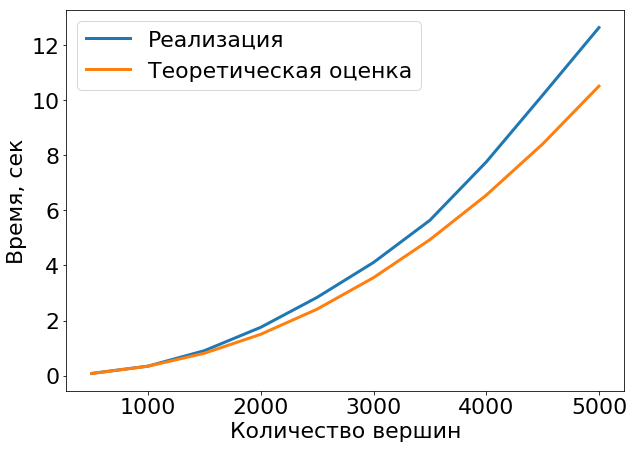
\includegraphics[width=\textwidth]{pics/plot_nconst}
                \caption{Без подбора константы}
                \label{fig:nonc}
            \end{subfigure}
            \begin{subfigure}[b]{0.49\textwidth}
                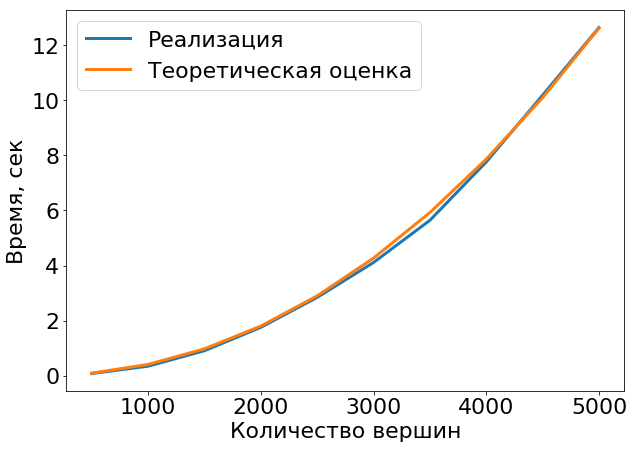
\includegraphics[width=\textwidth]{pics/plot_const}
                \caption{С подбором константы}
                \label{fig:cons}
            \end{subfigure}
            \caption{Время работы программы}
        \end{figure}

    \section{Реализация программы}
        Программа была реализована по алгоритмам, данных в книге \cite[разделы 21.3, 23.2]{clrs}. Также для удобства были написаны классы Edge и Graph. Edge -- реализация ребра, которая имеет операцию сравнения по весу. Graph -- реализация графа: умеет считывать с файла и записывать в файл граф.

        Компиляция: \verb|g++ main.cpp utils.cpp -o kruskal|

        \textbf{Вход программы}: файл содержащий список ребер построчно в формате:
        $$\textbf{город город расстояние}$$

        \textbf{Выход программы}: файл output.txt. Первая строка файла -- общая длина ребер покрывающего дерева, далее -- ребра формате <<город (номер) -- город (номер)>>.

        Запуск: \verb|./kruskal <путь до файла с данными>|.

        \quad Например \verb|./kruskal data/cities.txt|

    \begin{thebibliography}{9}
        \bibitem{clrs}
        Кормен Т.Х. и др. Алгоритмы: построение и анализ, 3-е изд., Москва, <<И. Д. Вильямс>>, 2016. -- 1328 с.
    \end{thebibliography}

\end{document}
